\chapter{Лоция}

\textbf{Морская лоция}\footnote{От голландского слова <<Loodsen>> \--- вести корабль.} родилась вместе с мореплаванием. В отличие от навигации или мореходной астрономии, основанных на математическом анализе, лоция носит описательный характер. Поэтому описание каждого конкретного океана, моря или их бассейнов также называется <<лоцией>>. В России первая лоция под названием <<Книга морская, зело потребная, явно показующая правдивое мореплавание на Балтийском море>> была издана в 1721~г. в Петербурге по указанию Петра~I.

Основная задача лоции \--- помочь мореплавателю избрать наиболее безопасный и выгодный путь для перехода морем. Для этого она даёт штурману сведения об опасностях в море, системах ограждения этих опасностей, знакомит его с метеорологическими условиями в районе плавания, даёт описание побережья и находящихся на нем портов, гаваней и бухт, указывает наиболее удобные курсы для переходов из порта в порт. Кроме того, лоция содержит все необходимые гидрологические и океанографические данные, характерные для описываемого района.

Обеспечение безопасности мореплавания возлагается на органы гидрографии. Так, в Великобритании этим занимается Гидрографический департамент Адмиралтейства, в Советском Союзе, \--- Главное управление навигации и океанографии Министерства обороны СССР (ГУНиО МО). Вместе с ГУНиО МО важную роль в обеспечении безопасности мореплавания играют специальные службы Министерства морского флота СССР \--- Главная морская инспекция, Гидрографическое предприятие, Службы безопасности мореплавания пароходств.

ГУНиО МО проводит научно\-/исследовательские работы в морях и океанах, собирает и систематизирует материалы для составления и корректуры морских карт и навигационных пособий, занимается ограждением морских опасностей, издаёт в качестве официальных пособий карты, лоции и другие руководства для мореплавания, а также систематически информирует мореплавателей об изменениях в навигационной обстановке по всем районам плавания.

В целях оказания помощи ГУНиО МО каждый судоводитель обязан немедленно сообщать его учреждениям о всех расхождениях карт, лоций и других пособий с действительностью: о вновь обнаруженных опасностях, об отсутствии на штатных местах знаков ограждения и случаях серьёзных неувязок при определении места судна по береговым предметам, о желательности нанесения на карту тех или иных местных приметных береговых сооружений, облегчающих опознание берега и т.\=,д. 

\section{Терминология морской лоции}

Как и любая другая наука, лоция имеет свою терминологию. Ниже приводятся основные термины.

\textbf{Оборудованная береговая полоса.}

\begin{description}
\item [Порт] (\textit{port})\footnote{В скобках даётся перевод терминов на английский язык} \--- место, закрытое от волнения, приспособленное для стоянки судов и имеющее средства для их разгрузки и погрузки, а также возможности для ремонта и снаряжения судов и обеспечения их необходимыми запасами (топлива, воды, продовольствия и пр.). Порты бывают военные, торговые и порты\-/убежища для стоянки во время шторма. 
\item [Рейд] (\textit{roadstead}) \--- любое пространство у берега, где судно может надёжно встать на якорь. Рейд считается открытым, если он не защищён от ветра и волнения хотя бы с одного направления. Рейд, расположенный в хорошо защищённой бухте, называется закрытым. 
\item [Гавань] (\textit{harbour}) \--- часть акваторий порта или рейда, закрытая от волнения, течения и ледохода искусственными сооружениями. В гавани судно может стоять у берега (причальной стенки или пирса). 
\item [Бассейн] (\textit{dock basin}) \--- общее наименование части акватории гавани или порта, ограниченной причалами, пирсами, молами. Изолированные бассейны в портах со значительным колебанием уровня воды под влиянием приливов и отливов называются доками. Доступ в док осуществляется через ворота (батопорты) или шлюзы. 
\item [Аванпорт] (\textit{outer harbour}) \--- внешняя часть порта или гавани, защищённая от волнения молами, волноломами или имеющая естественное укрытие. Аванпорт обычно имеет большие глубины, чем основная часть порта. 
\item [Дамба] (\textit{dam}) \--- гидротехническое сооружение в виде насыпи или вала, служащее для предохранения берега от затопления или размывания, а также для защиты каналов, рейдов и устьев судоходных рек от наносов и волнения. 
\item [Мол] (\textit{mole}) \---оградительное сооружение в портах и гаванях, примыкающее одним концом к берегу. Конечная часть мола, выступающая в море, называется головой мола. 
\item [Волнолом] (\textit{breakwater}) \--- внешнее, не связанное с берегом, оградительное гидротехническое сооружение для защиты рейдов или гаваней от волнения. 
\item [Пирс] (\textit{pier}) \--- причальное сооружение для судов, одним концом примыкающее к берегу. 
\item [Причал] (\textit{berth}) \--- место для стоянки судов в порту, оборудованное причальными приспособлениями \--- палами, кнехтами, тумбами. 
\item [Пал] (\textit{pawl, bit}) \--- 1.~Деревянная свая или куст свай, забитых в грунт. 2.~Чугунная тумба на причале, на которую заводят швартовы. 
\item [Фарватер] (\textit{fairway}) \--- безопасный путь плавания судов среди различного рода препятствий, ограждённый предостерегающими знаками. 
\item [Канал] (\textit{canal}) \--- искусственно прорытое русло для прохода судов через мелководье, обозначенное средствами навигационного оборудования. 
\end{description}

\textbf{Формы береговой черты.}

\begin{description}
\item [Бухта] (\textit{bay}) \--- небольшой залив. 
\item [Фиорд] (\textit{fiord}) \--- узкий глубокий залив или бухта, глубоко вдающиеся в гористые берега. 
\end{description}

\textbf{Навигационные опасности.}

\begin{description}
\item [Мель] (\textit{flat, ground}) \--- место, глубины над которым малы по сравнению с окружающими и поэтому опасные для мореплавания. 
\item [Отмель] (\textit{shoal}) \--- мель, простирающаяся от берега, с постепенно увеличивающимися глубинами. 
\item [Риф] (\textit{reef}) осыхающее или подводное возвышение морского дна со скалистым или коралловым грунтом; скопление камней, опасное для мореплавания. 
\item [Банка] (\textit{bank}) \--- отдельно лежащая мель, окружённая значительно большими глубинами. Считается безопасной для мореплавания, если глубина на ней более 20~м. 
\item [Бар] (\textit{bar of river}) \--- поперечная наносная мель в устьях рек или лежащая поперёк входа в бухту. 
\end{description}

\textbf{Грунты.}

\begin{description}
\item [Глина] (\textit{clay}) \--- плотный грунт. Совокупность мелких частиц размером Менее 0,001~мм. Обладает вязкостью, якорь держит хорошо. 
\item [Ил] (\textit{mud, slime, ooze}) \--- совокупность частиц меньше 0,01~мм. Бывает плотный, вязкий и жидкий. Якорь держит в зависимости от степени плотности. Плохо держит жидкий ил (ооzе). 
\item [Песок] (\textit{sand}), \textbf{гравий} (\textit{gravel}), \textbf{хрящ} \--- совокупность частиц размером от 0,5~мм (песок) до 5,0~мм (гравий) и крупнее (хрящ). Держащая сила \--- в зависимости от плотности. Обычно средняя. 
\item [Плита, твёрдый грунт] (\textit{hard ground}) \--- массивные горные породы. Как грунт держит очень плохо. 
\end{description}

\textbf{Навигационное оборудование.}

\begin{description}
\item [Веха] (\textit{spar buoy}) \--- плавучий предостерегающий знак для ограждения морских опасностей в виде деревянного или металлического шеста с поплавком, топовой фигурой или без неё, установленный на якоре. Может быть снабжена радиолокационным (уголковым или спиральным) отражателем. 
\item [Буй] (\textit{buoy}) \--- плавучий предостерегающий знак для ограждения морских опасностей или фарватеров в виде металлического поплавка с фермой, устанавливаемый на якоре. Буи могут иметь устройства для подачи туманных сигналов и освещения в тёмное время суток, иногда снабжаются пассивными радиолокационными или оптическими отражателями. 
\item [Бакен] (\textit{beacon}) \--- в отличие от буя не имеет фермы и обычно не освещается. 
\item [Маяк] (\textit{light house}) \--- навигационный ориентир в виде башни отличительной формы и окраски, устанавливаемый на материке, острове или непосредственно на мелководье, оснащённый осветительным устройством с большой оптической дальностью видимости. 
\item [Плавучий маяк] (\textit{lightship}) \--- судно, оборудованное маячным огнём и устанавливаемое в районе удалённых от берегов опасностей или перед входом в морской порт (с функциями лоцманской станции). 
\item [Створ] (\textit{leading line}) \--- линия или вертикальная плоскость, проходящая через два ориентира (створных знака) и указывающая мореплавателям безопасное направление для движения судна. Задний знак при наблюдении с моря должен быть выше переднего (рис.~\ris{54}). Створы могут быть ведущими, по которым судно идёт по заданному направлению; секущими, обозначающими место изменения курса на фарватере; девиационными, используемыми при работах по уничтожению девиации или определении поправки компаса. 
\end{description}

Перечисленные термины являются общепринятыми и употребляются в специальной литературе и официальных изданиях. В тех случаях, когда какой\-/либо термин не совпадает с местным названием предмета, в лоциях данного района обязательно указываются эти различия. 

\begin{figure}[htb]
  \centering{}
  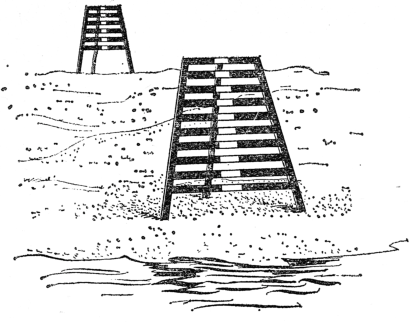
\includegraphics[scale=1.2]{0054P}
  \caption{Створные знаки}
  \label{fig:54}
\end{figure}

\section{Ограждение морских опасностей}

Для того чтобы обеспечить безопасность мореплавания, необходимо соблюдать по крайней мере два условия: с достаточной точностью нанести на навигационную карту все известные морские опасности и оградить эти опасности в море определёнными, хорошо видимыми знаками или другими искусственными предметами, по которым мореплаватель мог бы легко ориентироваться и заблаговременно уклониться от встречи с опасностью. Кроме того, каждый мореплаватель нуждается в различных береговых и морских ориентирах для определения своего места в море, опознания побережья, подходов к портам и якорным стоянкам.

Совокупность всех средств и устройств, которые обеспечивают безопасность мореплавания в определённом районе или море, обозначают надводную или подводную опасность, дают возможность опознать открывающийся берег и определить место судна при плавании вблизи берегов, называется навигационным оборудованием данного района или моря в целом. По месту установки средства навигационного оборудования могут быть береговыми и плавучими.

Основное назначение навигационного оборудования-ограждение морских опасностей. Плавучее ограждение устанавливают на воде \--- это буи, бакены, вехи и плавучие маяки, которые служат для непосредственного предостережения штурмана о существующей в данном месте опасности (рис.~\ris{55}). Береговое ограждение \--- морские и береговые маяки, береговые знаки и башни, створные знаки \--- устанавливают на прибрежной полосе материков и островов. В некоторых случаях роль берегового ограждения выполняют нанесённые на карту различные приметные места и предметы \--- отдельные высоты, триангуляционные вышки, приметные здания (церкви, башни и т.д.). 

\begin{figure}[htb]
  \centering{}
  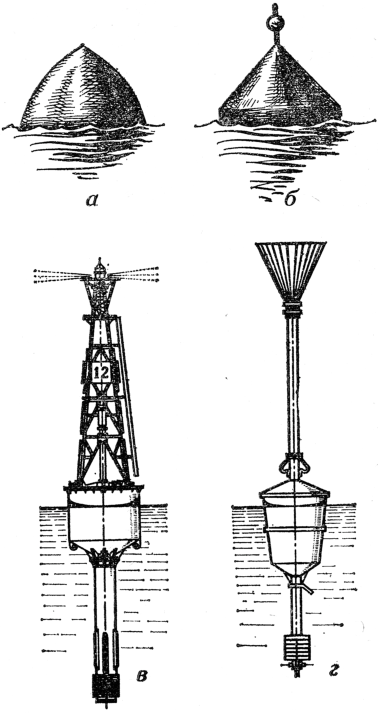
\includegraphics[scale=1.2]{0055P}
  \caption{Плавучее ограждение}
  \label{fig:55}
  \small
  \centering{}
  \textit{а, б} \--- Бакен; \textit{в} \--- буй; \textit{г} \--- веха
\end{figure}

По принятой в СССР единой системе ограждения, постоянные морские опасности делят на следующие группы:
\begin{enumerate}
\item Навигационные опасности 
  \begin{itemize}
  \item Естественные опасности (банки, мели, рифы, скалы и т.д.). 
  \item Кромки искусственных каналов и естественных фарватеров. 
  \item Затонувшие судна. 
  \item Районы свалки грунта. 
  \end{itemize}
\item Опасности не навигационного характера: 
  \begin{itemize}
  \item Опасные из-за мин районы и фарватеры в них; 
  \item Запретные для плавания районы и полигоны. 
  \item Районы рыбной ловли. 
  \end{itemize}
\item Прочие ограждаемые районы: 
  \begin{itemize}
  \item Кабели и мерные линии. 
  \item Карантинные и якорные места. 
  \end{itemize}
\end{enumerate}

Существует две системы плавучего ограждения перечисленных опасностей: латеральная и кардинальная.

\textbf{Латеральная система} основана на принципе расположения предостерегательных знаков \--- буев, бакенов, вех \--- справа или слева относительно сторон фарватера. Эта система применяется в основном при ограждении фарватеров, морских каналов, протраленных фарватеров в районах с минной опасностью, а также при ограждении судовых ходов на реках. Разновидностью латеральной системы можно считать ограждение широких фарватеров и рекомендованных курсов предостерегательными знаками вдоль осевой линии, дающее направление судну не <<между знаками>>, а <<от знака к знаку>>. Правая и левая стороны фарватера, обставленного по латеральной системе, определяются при следовании с моря (для морских и озёрных фарватеров).

\textbf{Кардинальная система} \-- её принцип основан на ограждении опасностей знаками, расставленными относительно сторон горизонта и указывающими мореплавателю, к какому из главных румбов (N, S, O или W) следует оставить буй или веху, чтобы миновать опасность. Эта система применяется при ограждении естественных навигационных опасностей, а также затонувших судов, запретных для плавания районов, районов свалки грунта, рыбной ловли и районов с минной опасностью. Все буи, как освещаемые, так и неосвещаемые, могут иметь и звуковые сигнальные устройства \--- колокола, ревуны, гудки. Эти устройства работают при волнении и служат для опознания буев в тумане. 

В водах Северо\-/Западной Европы с 1981~г. действует унифицированная система плавучих средств навигационного ограждения опасностей, которая в дальнейшем должна будет распространена на все районы Мирового океана. Эта система уже принята во всех государствах бассейна Северного моря, проливов Ла\-/Манш и Па\-/де\-/Кале, в Великобритании, Ирландии и на Атлантическом побережье Франции. Основана она на следующих принципах: 

\begin{itemize}
\item Возможность раздельного и совместного использования латеральной и кардинальной систем ограждения. 
\item Минимум числа плавучих знаков ограждения, их лёгкое и надёжное опознание по цвету и характеру огня, без применения секундомера. 
\item На латеральных знаках огни зелёные и красные, на кардинальных \--- белые, с резко отличающимися характеристиками. 
\item Затонувшие суда ограждаются, как и все другие навигационные опасности, кардинальными или латеральными знаками. 
\item Новые опасности ограждаются по этим же правилам. Внешний вид унифицированных знаков показан в приложении \ref{app:2}, \textit{д}. 
\end{itemize}

В унифицированной системе наименование кардинального знака, как в большинстве стран мира, означает сторону, с которой судно должно пройти его. В водах СССР переход на новую систему ограждения намечено осуществить в течение пяти лет: в 1981~г. \--- на Балтийском море, в 1982-1983~гг. \--- на Азовском и Чёрном морях, в 1984~г. \--- в морях Дальнего Востока и в 1985~г. \--- в морях Северного Ледовитого океана.

Область применения плавучих маяков намного меньше, чем других плавучих предостерегательных знаков. Как правило, плавмаяки устанавливают в районах морских опасностей, значительно удалённых от берега при входе в проливы, каналы или теры (например, плавмаяк <<Рижский>> в Рижском заливе), часто качестве приёмных маяков больших портов. Каждый плавучий маяк окрашивается приметным и отличным от краски других судов образом. Надводные борта плавмаяков обычно окрашиваются в красный цвет. Вдоль обоих бортов большими буквами пишется название маяка. Плавучий маяк, находящийся на своём штатном месте, должен нести на топе мачты решетчатый шар, а ниже него \--- маячный флаг жёлтого цвета с прямым синим крестом. Сорванный со своего штатного места плавмаяк считается неработающим и вместо шара и маячного флага должен нести: днем \--- по одному чёрному шару в носу и корме (или по одному красному флагу) ночью \--- по одному красному огню на тех же местах. Плавмаяки могут так же подавать туманные и другие сигналы. В последнее время плавмаяки выходят из употребления и заменяются башенными морскими маяками.

Плавучее ограждение называется \textbf{штатным}, если оно нанесено на карты, Дополнительное ограждение, выставляемое для каких-либо специальных целей в летнее время, называется \textbf{летним}. \textbf{Зимнее} ограждение выставляется после ледостава в замерзающих портах для обозначения входа и выхода из портов, а также участков и рейдов для безопасного движения ледоколов и проводимых ими караванов. О выставлении летнего или зимнего ограждения сообщается в <<Извещениях мореплавателям>>.

\begin{figure}[htb]
  \centering{}
  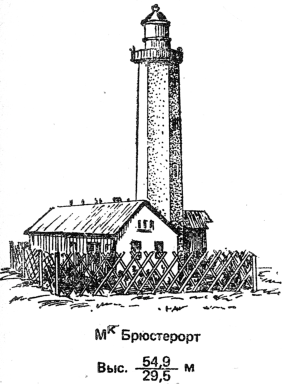
\includegraphics[scale=1.2]{0056P}
  \caption{Береговой маяк}
  \label{fig:56}
\end{figure}

\begin{figure}[htb]
  \centering{}
  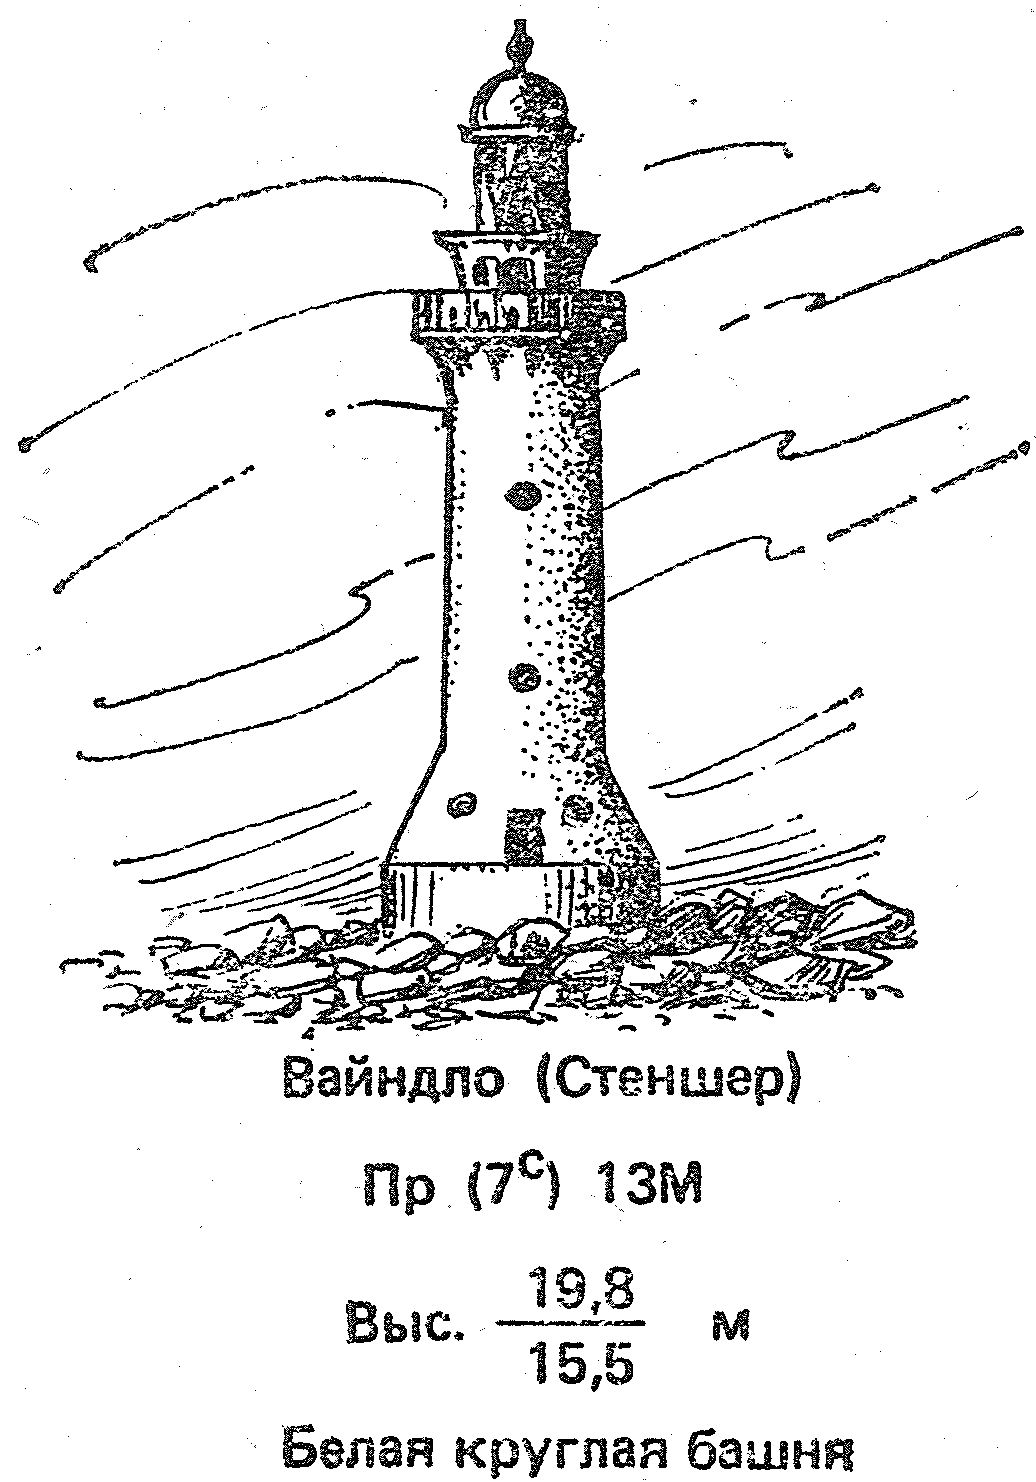
\includegraphics[scale=1.2]{0057P}
  \caption{Морской маяк}
  \label{fig:57}
\end{figure}


\begin{figure}[htb]
  \centering{}
  \includegraphics[scale=1.2]{0058P}
  \caption{Береговой знак}
  \label{fig:58}
\end{figure}


Средства \textbf{берегового ограждения} \--- маяки, освещаемые и неосвещаемые знаки, створы и т.\=,д. \--- устанавливают для того, чтобы облегчить мореплавателям ориентировку в море относительно морских опасностей, лучше опознать берег и вход в порт или на рейд, определить место судна при плавании в видимости берегов Основным береговым ориентиром является маяк. Оснащённый мощным источником света, маяк в хорошую погоду ночью имеет дальность видимости до 15\otdo 20 миль и более. Мореплаватели относятся к сигналам маяков с самой высокой степенью доверия, так как местоположение их неизменно. 

В отличие от других навигационных знаков маяк обслуживает мореплавателей круглые сутки и в любую погоду. В зависимости от места установки береговые маяки делят на собственно береговые и на морские. 

\textbf{Береговые маяки} возводят обычно на высоких, выдающихся в море мысах материка или больших островов (рис.~\ris{56}), \textbf{морские} \--- на расположенных вдали от берега естественных или искусственных островках или просто на подводной скале (рис.~\ris{57}). По своему назначению береговые маяки могут быть опознавательными (указательными) и створными. Первые, как видно из названия, обычно служат приёмным знаками при входе в какой-либо порт или канал (например, Дообский маяк при подходе к Новороссийску), поворотными знаками в том месте, где проходящие суда обычно меняют свой курс (например, Поворотный в Японском море), предостерегательными знаками, указывающими на определённую навигационную опасность (например, Родшер в Финском заливе). Створные маяки ставят для облегчения прохода судов в узкостях или входа на рейд, в гавань или в порт (например, Таллинские створные маяки).

Во избежание путаницы все маяки отличаются друг от друга не только внешним видом, но и характеристикой огня и туманного сигнала. Практически установлено, что маяки с одинаковой характеристикой не должны располагаться ближе чем в 80 милях друг от друга.

Главные требования к маякам сводятся к следующему: 

\begin{itemize}
\item Местонахождение каждого маяка должно быть точно нанесено на карту. 
\item Он должен быть хорошо виден и днем и ночью. 
\item Огонь маяка не должен приниматься за любой случайный огонь на берегу. 
\item Маяк должен иметь надёжную туманную сигнализацию. 
\end{itemize}

Кроме маяков на берегу устанавливают освещаемые и неосвещаемые знаки. Освещаемые знаки отличаются от маяков меньшей величиной и тем, что на них ставят автоматические источники света, менее мощные и не требующие постоянного обслуживания. Неосвещаемые знаки служат ориентирами только в дневное время (рис.~\ris{58}). 

\section{Сигнальные и другие станции}

Кроме знаков плавучего и берегового ограждения безопасность мореплавания обеспечивает ряд специальных сигнальных станций, задача которых \--- передача на суда, находящиеся в море, сведений, имеющих значение для безопасного плавания. Они могут находиться при маяках или работать самостоятельно. К таким станциям относятся прежде всего радиостанции, которые в зависимости от своего назначения передают метеорологические сводки, радионавигационные извещения, сигналы времени и медицинские советы. Эти передачи ведутся по установленной программе, по запросу или в определённое время суток. 

\textbf{Телефонные станции} при маяках позволяют связать их с ближайшим портом или населённым пунктом.
Метеосводки и радионавигационные извещения (сокращённо МЕТЕО и НАВИМ) информируют мореплавателей об ожидаемой погоде и изменениях в навигационной обстановке. Их передают все береговые станции Министерства морского флота открытым текстом. Эти извещения могут быть очередными и срочными. Последние передаются немедленно по поступлении на радиостанцию, а очередные \--- по расписанию передач. Сигналы времени по радио даются в соответствии с программой, установленной данной станции, подробности о которой указываются в лоциях и в специальном издании <<Радиосигналы времени>>.

Кроме радиосвязи для передачи на суда нужной информации используются также звуковые, флажные (фигурные) и световые средства сигнализации. Для подачи таких сигналов на хорошо видном с моря месте устанавливают сигнальные посты, оборудованные мачтой, на которой поднимаю определённые сочетания флагов или фигур, обозначающих необходимы сигналы. В тёмное время суток эти сигналы передаются азбукой Морзе помощью клотикового фонаря или сочетаниями красного, зелёного и белого огней. С сигнальных постов обычно подаются следующие сигналы:
\begin{description}
\item [<<Предупреждение об опасности>>] \--- подаётся плавучими маяками, на мачте которых для судов, чей курс ведёт к опасности, поднимается двухфлажный сигнал по Международному своду сигналов \--- <<Вы идёте к опасности>> с одновременным пуском ракет (ночью сигнал даётся только ракетами). Сигнал подаётся до тех пор, пока судно не увидит его и не изменит своего курса.
\item [<<Лоцманские сигналы>>] \--- они регулируют движение судов по каналу или фарватеру, сообщают о глубинах на фарватерах, о приливах и отлива в порту, о течениях и о высоте воды и т. п.
\end{description}

\textbf{<<Штормовые сигналы>>} \--- для предупреждения мореплавателей и населения портовых городов о надвигающихся штормах и сильных ветрах. Эти сигналы имеют значение для ограниченного района и служат в основной предупреждением для выходящих в море судов (см. приложение~\ref{app:2}, \textit{е}).

Туманные сигналы, имеющие весьма серьёзное значение для безопасности плавания вблизи берегов, подают воздушными и подводными средствами звуковой сигнализации при снижении видимости (туман, снежный заряд, морозь и т.\=,п.). В советских водах воздушные туманные сигналы подаются береговыми маяками при помощи следующих устройств: 

\begin{description}
\item [наутофон] \-- мембранный излучатель со звуком, напоминающим звук горна. Дальность слышимости достигает 3\otdo 4 миль; 
\item [сирена] \--- паровая или пневматическая с неподвижным или вращающимся рупором. Издаёт сильный воющий звук и имеет среднюю дальность слышимости 6\otdo 8 миль; 
\item [диафон] \--- издаёт сильный прерывистый звук, слышимый на расстоянии 6\otdo 8 миль;
\item [туманный горн] \--- имеет однотонный звук с небольшой дальностью слышимости (до 2 миль). Применяется в основном на плавучих маяках;
\item [свисток (или ревун)] \--- применяется на морских буях. Работает автоматически при волнении определённой силы;
\item [пушка] \--- выстрелы производятся с промежутком 10~мин. При ветре с моря выстрелы даются чаще;
\item [взрывы] \--- сильный звук от взрыва специального патрона на большой высоте; распространяется во все стороны и считается надёжнее пушки;
\item [колокол] \--- в настоящее время применяется только на морских буях в качестве дублирующего средства на маяках.
\end{description} 

Береговые маяки подают двухударный звон с промежутком до 3 мин; плавучие маяки \--- трёхударный звон с промежутком до 2 мин.

Отдельно могут быть выделены \textbf{радиопеленгаторные станции и радиомаяки}, которые, передавая определённые сигналы, служат для определения места судна в море при помощи радиопеленгов.

\textbf{Лоцманские станции} обеспечивают лоцманскую проводку судов в порт и из порта, а \textbf{спасательные станции} оказывают помощь судам, терпящим бедствие.

Все сведения о маяках, сигнальных станциях и передаваемых ими сигналах даются в <<Лоциях>> и отдельных изданиях <<Огни и знаки>> по каждому морю. В этих же изданиях имеются данные о лоцманских и спасательных станциях. Пункты, где имеются такие станции, обозначают на картах.

\section{Морские карты}\label{sec:maps}

\textbf{Морские карты} \--- основное пособие каждого штурмана. По своему назначению карты делятся на две основные группы: навигационные, непосредственно используемые в судовождении, и справочные \--- сборные листы, карты ветров, течений, часовых поясов, радиомаяков и т. д. К навигационным относятся следующие карты: 

\begin{description}
\item [генеральные (общие) карты,] которые имеют масштаб от 1\=,:\=,500\=,000 до 1\=,:\=,5\=,000\=,000 и служат для общего изучения изображаемых на них морей, океанов и их частей и для нанесения предварительной прокладки. На генеральных картах показывают только главные маяки и огни. Освещаемые буи и дневное плавучее ограждение наносят только у внешних опасностей и на подходах к портам. Изобаты нанесены по глубинам 20, 50, 100 и 200~м; 
\item[путевые карты,] масштаб которых от 1\=,:\=,100\=,000 до 1\=,:\=,500\=,000, служат для ведения навигационной прокладки и определения места судна с достаточной для мореплавания точностью. Внешние средства навигационного обеспечения наносят на этих картах полностью, а внутри рейдов и портов с большой разрядкой. Изобаты нанесены по глубинам 5, 10, 20, 50 и 100~м; 
\item[частные карты,] которыми пользуются для прокладки при плавании в непосредственной близости от берегов, в шхерах и узкостях и при подходе к берегу. Они имеют масштабы от 1\=,:\=,25\=,000 до 1\=,:\=,75\=,000. Изобаты нанесены по глубинам 2, 5, 10, 20, 50~м и все навигационные опасности с их береговым и плавучим ограждением; 
\item[планы] дают подробные изображения портов, бухт, гаваней, якорных стоянок и других ограниченных акваторий. Масштаб планов от 1\=,:\=,500 до 1\=,:\=,25\=,000. Все навигационные ограждения на планах наносят полностью. 
\end{description}

Для того чтобы правильно пользоваться картой, надо уметь читать её, т.\=,е. понимать все нанесённые на карту условные обозначения и правильно разбираться в них. Чтение карты следует начинать с заголовка, в котором указывается её название (район плавания), числовой масштаб с указанием главной параллели, к которой он отнесён, меры, в которых даны глубины и высоты прибрежных гор, а также год, к которому приведено магнитное склонение. После заголовка прочитывают расположенные под нижней рамкой отметки о датах последней (большой и малой) корректуры данной карты и год её издания.
 
Все примечания, предупреждения (печатающиеся красным цветом), рисунки маяков и планы портов помещаются на карте таким образом, чтобы не закрывать береговой черты и водной поверхности. Адмиралтейский номер карты проставляется во всех четырёх углах. С 1968~г. номера советских морских карт состоят из пяти цифр. Первая из них обозначает район Мирового океана, вторая \--- масштаб карты, третья \--- район океана или море, последние две цифры \--- порядковый номер карты данного района океана или моря. 

После предварительного знакомства с картой подробно просматривают район, в котором предстоит плавать, чтобы во всех подробностях изучить навигационную обстановку \--- глубины, опасности и систему их ограждения, береговую черту, расположение маяков и знаков. 

Для изображения на карте состояния и особенностей поверхности моря его дна и побережья применяется система условных обозначений, приведённая в приложении~\ref{app:2}, \textit{а}. 

\textbf{Глубины} на современных картах показываются в метрах и дециметрах. Точки с одинаковыми глубинами соединяются линиями равных глубин \--- изобатами. Изобата отделяющая прибрежное мелководье либо отдельную мель или банку, называется \textbf{линией опасности}, или \textbf{предостерегательной изобатой}. Для малых судов линией опасности считается 10-метровая изобата. 

Грунты обозначаются условными сокращениями, например: \textit{П} \--- песок, \textit{И} \--- ил, \textit{Кор} \--- кораллы и т.\=,д. Сложные грунты указывают сочетаниями сокращений составляющих грунтов: \textit{ИП} \--- илистый песок, \textit{ГрП} \--- гравий с песком, \textit{СрГл, МК} \--- серая глина, мелкий камень. Буквами обозначаются также цвет и характеристика грунта: \textit{жлП} \--- жёлтый песок, \textit{срмПГл} \--- серый мелкий песок с глиной. Если составляющие грунта располагаются слоями, то первым пишется верхний слой \textit{мППл} \--- мелкий песок на плите. 

\textbf{Естественные навигационные опасности} \--- банки, мели, рифы дают на картах контуром из точек с обязательным указанием наименьшей глубины над ними. Все остальные морские опасности обозначаются различными условными знаками. Если положение или существование показанной на карте опасности вызывает сомнения, то рядом с обозначением такой опасности или внутри неё ставятся пометки: \textit{ПС} \--- <<положение сомнительно>> или \textit{СС} \--- <<существование сомнительно>>. 

Места якорных стоянок обозначаются рисунком якоря. Изображение якоря без штока означает стоянку для малых судов, а якоря со штоком \--- для больших судов. Район с плохим грунтом обводят пунктиром с надписью: \textit{плх} (плохой грунт). 

Величина магнитного склонения указывается либо в заголовке карты, если она одинакова для всей карты, либо в центре картушки, расположенной на водной поверхности карты; центр картушки совмещается с точкой, где было определено склонение. В этой же картушке указывается годовое изменение склонения. Иногда величины склонений дают и без картушек. Так как картушки склонений имеют истинные направления, ими можно пользоваться вместо транспортира. Районы магнитных аномалий обводят сплошной толстой линией. 

Почти все средства навигационного оборудования имеют свои условные знаки. То, что не имеет своего знака, обозначается кружком с точкой в центре. Эта точка на карте соответствует точному местоположению знака на местности. Освещаемые знаки и маяки имеют на карте цветные изображения огней и их характеристики. Расцветка маячных огней показывается цветными окружностями с центром в точке нахождения маяка или частями окружности в пределах угла освещения. Характеристика огня даётся рядом с маяком в одну строчку, например: \textbf{ГрПр(3)(25с)10М(н)}, что означает \--- группопроблесковый огонь с тремя проблесками и периодом 25~с, Дальность видимости 10~миль, туманный сигнал \--- наутофон. 

Направления, обозначающие граниты углов освещения маяков, на картах читаются от маяка в море. 

Створы обозначают на картах \textbf{сплошными линиями} (ходовая часть) и \textbf{пунктиром} (неходовая часть, а также поворотные и секущие створы на мерных линиях).

\textbf{Морские течения}, которые необходимо учитывать при прокладке, наносят на карты в виде стрелок: показывающие направление постоянного течения \--- с оперением, переменное \--- волнистой линией. Скорость течения с точностью до 1/4~уз пишется сверху стрелки. Приливные течения обозначают стрелкой с оперением сверху, отливные \--- без оперения (см. рис.~\ris{125}). 

Различные \textbf{приметные строения и предметы на берегу}, чьё место определено, \--- церкви, башни, отдельные высоты, \--- также показывают условными знаками. Точное место показанного на карте предмета относится к середине основания или к центру условного знака. 

Представляющие для мореплавателя серьёзную опасность \textbf{затонувшие суда} обозначаются пятью различными знаками: для затонувших судов с частями корпуса, возвышающимися над водой и представляющими явную опасность; с мачтами над водой; для судов, глубина над которыми меньше 18~м и больше 18~м; осыхающих. 

При подборе карт для плавания необходимо иметь в виду, что для прокладки следует использовать только карты самого крупного масштаба и откорректированные по день выхода в море. Корректура карт \--- это нанесение на неё тех изменений в морской и навигационной обстановке, которые произошли со дня её издания: вновь обнаруженные опасности, упразднение одних знаков навигационной обстановки и открытие других, результаты новых промеров и т.\=,д., о которых должен знать мореплаватель. 

Большая корректура нужна при появлении новых гидрографических данных или накоплении большого числа малых корректур, которые существенно изменяют оригинал карты. Поэтому большая корректура проводится только картографическим производством \--- издаются новые исправленные карты. 

Малая корректура обычно предусматривает незначительные изменения. Её выполняют от руки красными чернилами или тушью. Малая корректура карт, находящихся на складе гидрографии, производится работниками гидрографии, а карт, имеющихся на судах, \--- штурманами на основании <<Извещений мореплавателям>> (в плавании \--- по радиоизвещениям НАВИМ). Дата последней корректуры на получаемых из гидрографии картах должна быть указана под нижней рамкой карты со ссылкой на номера использованных <<Извещений мореплавателям>>. 

\section{Навигационные пособия}

Кроме морских карт в практике судовождения используют различные навигационные пособия, и в первую очередь <<Лоции>>, которые дополняют и уточняют сведения, данные на картах, облегчая тем самым решение навигационных задач. Кроме <<Лоций>> ГУНиО МО СССР издаёт и другие, вспомогательные, пособия: <<Каталог карт и книг>>, книги <<Огни и знаки>>, справочники <<Радиомаяки>>, различные таблицы и бланковые издания, в том числе и книгу <<Условные знаки морских карт и карт внутренних водных путей>>. 

\textbf{<<Лоции>>} издают отдельно для каждого моря или части океана. В общем случае каждая книга <<Лоции>> состоит из четырёх основных разделов: 

\begin{enumerate}
\item \textbf{общий обзор}, в котором содержатся сведения о границах описываемого района, навигационно\-/географические и гидрометеорологические данные, сведения о портах и якорных стоянках, а также правила плавания в иностранных водах; 
\item \textbf{навигационное описание}, которое для удобства разделено по районам, и содержащее последовательно отдельные участки побережья, заливы, проливы, порты, фарватеры, приметные места, морские опасности, а также дающее наставления для плавания в различных местах, имеющих какие-либо особенности;
\item \textbf{справочный отдел}, где имеются таблицы расстояний между портами, словарь местных и иностранных слов и терминов, встречающихся в <<Лоции>> и на картах, и другие сведения; 
\item \textbf{алфавитный указатель}, содержащий географические названия всех портов, мысов, проливов, заливов, якорных стоянок и т.\=,п. Если <<Лоция>> охватывает иностранные воды, алфавитный указатель состоит из двух частей, в которых названия даются в русской и латинской транскрипции. 
\end{enumerate}

Кроме письменного материала <<Лоция>> содержит фотографии и рисунки приметных береговых мест и сборный лист карт данного района или моря. 

Так как срок службы <<Лоции>> около 10 лет, в течение этого времени периодически выпускаются дополнения и изменения, содержащие корректурный материал. Обязательным документом для корректуры <<Лоций>> являются также <<Извещения мореплавателям>>. Учёт корректуры ведётся на специальном листе, вклеенном в самом начале книги. 

<<Огни и знаки>> издаются чаще <<Лоций>> (через каждые 3\otdo 5~лет) и служат постоянным дополнением к ним. Их выпускают для каждого моря отдельно. Здесь есть все нужные штурману данные о маяках, освещаемых знаках, огнях и буях. Для получения этих данных надо найти в алфавитном указателе по названию маяка его номер, по которому и отыскивают сам маяк. О каждом маяке книга <<Огни и знаки>> сообщает следующие сведения: номер; название; положение (где находится маяк); широту и долготу с точностью до одной минуты; число, цвет, характер огня; дальность видимости огня (огней) в ясную погоду (в милях); высоту огня от уровня моря и от основания маяка (в метрах); описание маяка, его вид и окраску, высоту сооружения от его основания (в метрах); дополнительные сведения. 

Как и <<Лоции>>, книги <<Огни и знаки>> нуждаются в своевременной корректуре, основанием для которой служат <<Извещения мореплавателям>>. Кроме того, по мере накопления материала периодически издаются <<Дополнения к книгам ,,Огни и знаки''>>. 

<<Извещения мореплавателям>> \--- основные документы для корректуры карт и пособий \--- издают для всех морей Советского Союза и тех иностранных вод, которые охвачены советскими картами и пособиями, а также отдельно для районов плавания в советских водах, обслуживаемых Гидрографической службой флотов. Каждое <<Извещение мореплавателям>> имеет свой порядковый номер и ссылку на документ, по которому оно объявляется. 

Вспомогательным пособием для штурмана является <<Каталог карт и книг>>, который содержит подробные сведения о картах и навигационных пособиях и служит для подбора карт и пособий к предстоящему плаванию. Для того чтобы подобрать карту или <<Лоцию>>, пользуются сборными листами, помещёнными в каталоге. 

<<Радиотехнические средства навигационного оборудования>> содержат сведения о морских радиомаяках и радионавигационных системах, о радиостанциях, передающих МЕТЕО и НАВИМ. 

Кроме этих пособий ГУНиО МО СССР издаёт также <<Мореходные таблицы>> (МТ) и <<Морские астрономические ежегодники>> (МАЕ), служащие для решения навигационных и астрономических задач.
